\documentclass{article}
\usepackage{graphicx} % Required for inserting images
\usepackage{mathtools, nccmath}
\usepackage{hyperref}
\usepackage{apacite}
\usepackage{amsfonts}
\usepackage[mathscr]{eucal}


% \title{Credit Card Fraud detection using ML and HE}
% \date{April 2023}

\begin{document}

\begin{titlepage}
   \begin{center}
       \vspace*{1cm}

       \textbf{\Large{ELEMENTS OF CRYPTOGRAPHY}}

       \vspace{0.5cm}
        \large{Credit Card Fraud detection using ML and HE}
            
       \vspace{1.5cm}

       

       \vfill
            
       \textbf{ Group Members}\\
            
       \vspace{0.8cm}
     
       % \includegraphics[width=0.4\textwidth]{university}
            
       Meet Bhatt (202001267)\\
       Vraj Chaudhari (202003006)\\
       Jay Patel (202003019)\\
       Kunjera Shreyansh (202003031)
            
   \end{center}
\end{titlepage}

\begin{center}
    \textbf{CONTRIBUTION:}
\end{center}

\begin{itemize}
    \item \textbf{Meet Bhatt:} Gathering the information related to our encryption scheme, Analysis on Dataset, Creating SRS.
    \item \textbf{Chaudhari Vraj:} Analysis on Dataset, Implementation of code, Creating PPT, Report and Video.
    \item \textbf{Jay Patel:} Analysis of encryption scheme, Implementation of code, Creating PPT, Report and Video.
    \item \textbf{Shreyansh Kunjera:} Analysis on Dataset, Implementation of code, Creating PPT, Report and Video.
\end{itemize}

\pagebreak

\section{Introduction}

In the financial sector, detecting credit card fraud is a major issue that may be solved in a number of ways, one of which is by using machine learning algorithms. The need to secure sensitive financial data from unauthorised access is a barrier when applying machine learning algorithms for fraud detection. A cryptographic method named as homomorphic encryption enables us to do computations on encrypted data without having to first decrypt it, protecting the confidentiality and security of the sensitive data.

% \noindent Here is a general outline of how one could use homomorphic encryption and machine learning for credit card fraud detection:

% \begin{itemize}
%     \item Data collection: Collect a large dataset of credit card transactions that include both fraudulent and legitimate transactions. 
%     \item Data preprocessing: Preprocess the data by cleaning and transforming it into a format suitable for machine learning algorithms. This might involve data normalization, feature engineering, and data partitioning into training and testing sets.
%     \item Homomorphic encryption: Apply homomorphic encryption to the data to protect the sensitive financial information.
%     \item Machine learning: Use a machine learning algorithm to train a model to distinguish between fraudulent and legitimate transactions. Since the data is encrypted, the machine learning algorithm must be capable of processing the encrypted data.
%     \item Model evaluation: Evaluate the performance of the machine learning model using the testing data set. 
%     \item Deployment: Once the model is trained and evaluated, it can be deployed into production to automatically detect fraudulent transactions in real-time.
% \end{itemize}

% Overall, using homomorphic encryption and machine learning for credit card fraud detection can help protect sensitive financial data while still allowing for accurate fraud detection. However, it is important to keep in mind the limitations of homomorphic encryption, such as the potential for increased computational complexity and slower processing times compared to non-encrypted data.


\section{Homomorphic Encryption}

\noindent Homomorphic encryption(HE) is an encryption scheme which allows us to perform mathematical operations on encrypted data. In other words, HE allows computation on ciphertext, while maintaining the confidentiality of the plaintext (unencrypted data).

\begin{center}
    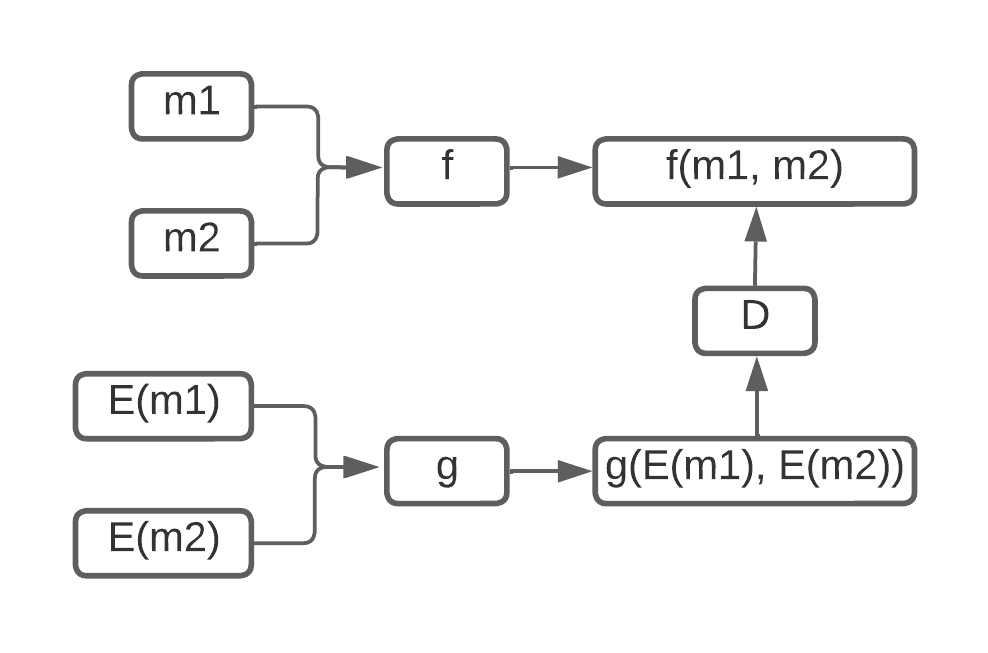
\includegraphics{Homomorphic2.png}
\end{center}

\noindent Homomorphic encryption can be applied in various scenarios, such as secure computation in cloud computing, privacy-preserving data analysis, and secure multiparty computation. It has the potential to enable secure computation on sensitive data without the need to reveal the data in plaintext, which is particularly useful for protecting user privacy.

\noindent There are various types of HE encryption techniques, such as fully homomorphic encryption (FHE) and partially homomorphic encryption (PHE). FHE allows arbitrary computation on encrypted data, while PHE only enables certain types of computations, such as addition or multiplication. However, FHE is currently less efficient and more computationally expensive than PHE.

\noindent HE can be used in machine learning to enable secure computation on sensitive data while preserving the confidentiality of the user data. This is particularly useful in scenarios where multiple parties want to collaboratively train a ML model without revealing their users private data to each other.


\section{CKKS}
% # rounding off, LWE, main motive
\noindent CKKS is not a perfect HE(Homomorphic Encryption) scheme. It is an Approximate HE. The goal of ckks is to find the efficient approximation of computation on HE. The key concept is to interpret encryption noise as an error that can happen when performing approximate computations. In other words, if a message is encrypted using the secret key $sk$, the decryption structure will be of the type $\langle c, s_k \rangle = m + e $(mod $q$), where $e$ is a minor error added to ensure the security of the hardness assumptions. If $e$ is sufficiently small in relation to the message, this noise is unlikely to affect the significant figures of m, and the approximation arithmetic value $m' = m + e$ can take the place of the original message. Before encryption, one can multiply the message by $\Delta$(scaling factor)  to decrease the precision loss caused by encryption noise.

% Add photo of overview of how the whole CKKS works\\

\begin{center}
    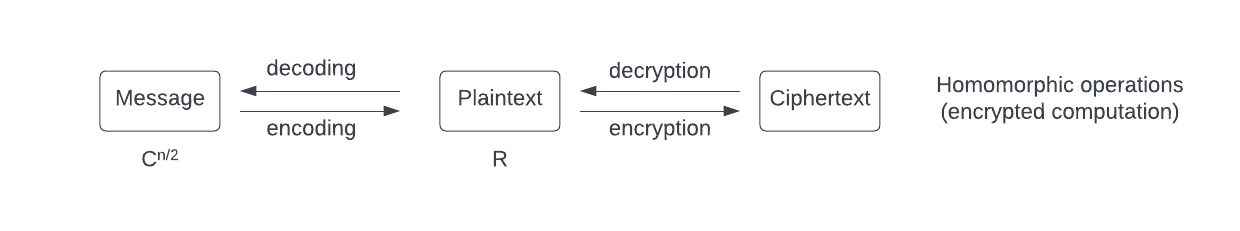
\includegraphics[scale = 0.6]{Crypto_Img_1.png}
\end{center}

\noindent In order to ensure that the result is smaller than $q$(ciphertext modulus) for homomorphic operations, we keep our decryption structure small enough in relation to the $q$. The fact that a message's bit size increases exponentially with circuit depth without being rounded remains a problem, nevertheless. We propose a novel ciphertext message manipulation method termed as rescaling to solve this issue.   \\

\noindent We have used Microsoft’s Tenseal library for Homomorphic Encryption whose brief introduction is given below

\subsection{Microsoft Tenseal Library}

\noindent We have used TenSEAL to implement CKKS encryption. TenSEAL is used to perform HE operations on tensors. It is constructed on top of Microsoft Tenseal, a C++ library that implements the HE algorithms BFV and CKKS. TenSEAL is a C++ library with a Python interface that offers simplicity through a Python API while maintaining efficiency by carrying out the majority of its operations in C++.



\subsection{Why to use CKKS ?}

\noindent One must manage enormous amount of data collections because a lot of data is generated in a cloud computing environment. Our technique may be a useful tool for data analysis, due to its ability to encrypt a huge amount of data into a single ciphertext and parallelize both computation and space. For instance, we used a batching technique to enhance the evaluation of the logistic function.


\subsection{Encoding and Decoding}

\noindent For effective homomorphic computation, a vector of several plaintexts must inevitably be encrypted in a single ciphertext. A ring isomorphism could be used to decode a plaintext polynomial as a vector of plaintext values into a product of finite fields. After performing homomorphic operations, an inserted error is positioned apart from the plaintext space so it can be eliminated using the plaintext characteristic.     \\

\noindent The plaintext of our approach, on the other hand, is a component of a cyclotomic ring with the property zero, and it includes a minor error that is either added during encryption to assure security or occurs during approximation arithmetic. Therefore, we adapt the complex canonical embedding map, an isometric ring homomorphism. In order to prevent a little inaccuracy in a plaintext polynomial from having a big impact on the encoding and decoding processes, it maintains the size of polynomials.
\\

\noindent $\textbf{Ecd}(z ; \Delta)$. Let $z=\left(z_i\right)_{i\in T}$ be a $(N/2)$-dimensional vector of complex numbers, the encoding procedure expands it into the vector $\pi^{-1}(z) \in \mathbb{H}$ and computes its discretization to $\sigma(\mathcal{R})$ after multiplying $\Delta$ (scaling factor). Return integral polynomial

\begin{equation*}
m(X)=\sigma^{-1}\left(\left\lfloor\Delta \cdot \pi^{-1}(z)\right\rfloor_{\sigma(\mathcal{R})}\right) \in \mathcal{R}
\end{equation*}


\noindent $\textbf{Dcd}(m ; \Delta)$. Let $m \in \mathcal{R}$ be an input polynomial, return the vector $z=\pi \circ \sigma\left(\Delta^{-1} \cdot m\right)$, i.e., the $j^{th}$ entry in $z$ is $\in T$ is $z_j=\Delta^{-1} \cdot m\left(\zeta_M^j\right)$.
\\

% Add photo of how encoding of plaintext works\\

\begin{center}
    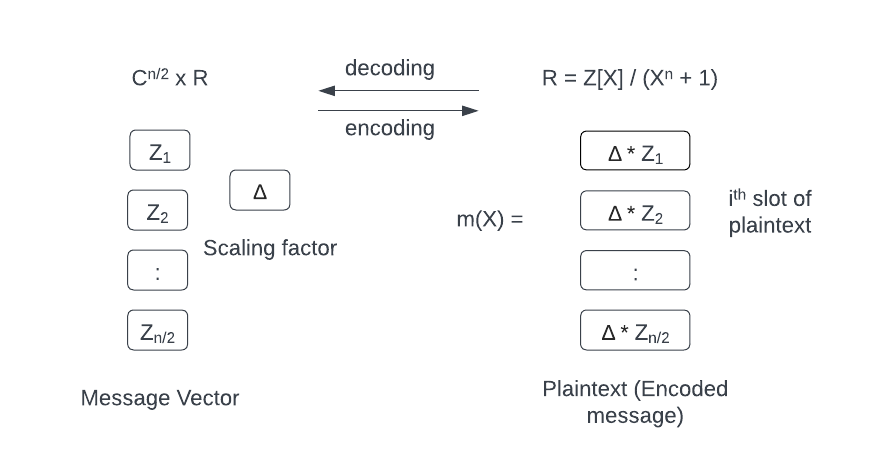
\includegraphics[scale = 0.8]{Crypto_Img_4.png}
\end{center}

\noindent We can encrypt several messages in a single ciphertext using the batching mechanism in the HE system, which also allows for parallel processing. In real world, we use it as an advantage to parallelize computations and decrease their complexity and memory requirements.




\subsection{Encrypt and Decrypt}

% The purpose of this subsection is to construct a leveled HE scheme for approximate arith- metic.Forconvenience,wefixabasep>0andamodulusq0,andletql =pl·q0 for0<l≤L. The integer p will be used as a base for scaling in approximate computation. For a security parameter λ, we also choose a parameter M = M(λ,qL) for cyclotomic polynomial. For a level 0 ≤ l ≤ L, a ciphertext of level l is a vector in Rkql for a fixed integer k. Our scheme consists of five algorithm (KeyGen, Enc, Dec, Add, Mult) with constants Bclean and Bmult(l) for noise estimation. For convenience, we will describe a HE scheme over the polynomial ring R = Z[X]/(ΦM(X)).

% KeyGen(1λ). Generate a secret value sk, a public information pk for encryption, and a evaluation key evk.
% Encpk(m). For a given polynomial m ∈ R, output a ciphertext c ∈ RkqL. An encryption c
% of m will satisfy ⟨c, sk⟩ = m + e (mod qL) for some small e. The constant Bclean denotes
% an encryption bound, i.e., error polynomial of a fresh ciphertext satisfies ∥e∥can ≤ B
% ∞ clean
% with an overwhelming probability.
% • Decsk(c). For a ciphertext c at level l, output a polynomial m′ ← ⟨c,sk⟩ (mod ql) for
% the secret key sk.
% The algorithms for homomorphic operations are required to satisfy the following proper- ties.
% Add(c1,c2).Forgivenencryptsofm1 andm2,outputanencryptionofm1+m2.Anerror of output ciphertext is bounded by sum of two errors in input ciphertexts.
% Multevk(c1,c2). For a pair of ciphertexts (c1,c2), output a ciphertext cmult ∈ Rkql which
% satisfies ⟨cmult, sk⟩ = ⟨c1, sk⟩ · ⟨c2, sk⟩ + emult (mod ql) for some polynomial emult ∈ R
% with ∥e ∥can ≤ B (l). mult ∞ mult
% RSl→l′(c). For a ciphertext c ∈ Rkql at level l and a lower level l′ < l, output the
% ciphertext c′ ← jql′ cm in Rk , i.e., c′ is obtained by scaling ql′ to the entries of c and rounding the coefficients to the closest integers. We will omit the subscript l → l′ when l′ =l−1.  \\

\noindent Constructing a leveled HE scheme for approximate arithmetic is the purpose of this section. For convenience, we fix a modulus $q_0$ and a base $0 < p$ , and let $q_\ell=p^\ell \cdot q_0$ for $0<\ell \leq L$. $p$ is used as a base for scaling. For a security parameter $\lambda$, we choose a parameter $M=M\left(\lambda, q_L\right)$ for cyclotomic polynomial. For a level $0 \leq \ell \leq L$, a ciphertext of level $\ell$ is a vector in $\mathcal{R}_{q\ell}^k$ for a fixed integer $k$. Our cryptographic scheme has five algorithms (Addition, Multiplication, KeyGeneration, Encryption, Decryption). We will be describing a HE scheme over polynomial ring $\mathcal{R} = \mathbb{Z}[X] / (\Phi_M(X))$
\\

\begin{itemize}
    \item \textbf{KeyGeneration} $\left(1^\lambda\right)$. Creates a secret key $s_k$, a public key $p_k$, and a evaluation key $evk$.
    
    \item $\textbf{Encryption}_{pk}(m)$. For a given polynomial $m \in \mathcal{R}$, return a ciphertext $c \in \mathcal{R}_{q_L}^k$. An encryption $c$ of $m$ will satisfy $\langle c, s k\rangle=m+e\left(\bmod q_L\right)$ for some small $e$. 
    
    % The constant $B{\text {clean }}$ denotes an encryption bound, i.e., error polynomial of a fresh ciphertext satisfies $\|e\|{\infty}^{\text {can }} \leq B{\text {clean }}$ with an overwhelming probability.
    
    \item $\textbf{Decryption}_{sk}(c)$. For a ciphertext $c$ at level $\ell$, output a polynomial $m^{\prime} \leftarrow\langle c, s k\rangle\left(\bmod q{\ell}\right)$ for $s_k$.
    
    \item $\textbf{Addition}\left(c_1, c_2\right)$. are encryptions of $m_1$ and $m_2$, output an encryption of $m_1+m_2$. 
    
    % An error of output ciphertext is bounded by sum of two errors in input ciphertexts. satisfies $\left\langle c_{\text {mult }}, s k\right\rangle=\left\langle c_1, s k\right\rangle \cdot\left\langle c_2, s k\right\rangle+e_{\text {mult }}\left(\bmod q_{\ell}\right)$ for some polynomial $e_{\text {mult }} \in \mathcal{R}$ with $\left\|e_{\text {mult }}\right\|{\infty}^{\text {can }} \leq B{\text {mult }}(\ell)$.

    \item $\textbf{ReScaling}_{\ell \rightarrow \ell^{\prime}}(\mathbf{c})$. Let $c \in \mathcal{R}_{q{\ell}}^k$ be a ciphertext, at level $\ell$ and $\ell '$a lower level, output $c^{\prime} \leftarrow\left\lfloor\frac{q{\ell^{\prime}}}{q_{\ell}} c\right\rceil$ in $\mathcal{R}_{q{\ell^{\prime}}}^k$, i.e., $c^{\prime}$ is a ciphertext obtained by scaling $\frac{q_{\ell^{\prime}}}{q_{\ell}}$ to the entries of $c$ and rounding the coefficients to the closest integers. We will omit the subscript $\ell \rightarrow \ell^{\prime}$ when $\ell^{\prime}=\ell-1$.
\end{itemize}


\subsection{Rescaling}

\noindent The rescaling process produces a ciphertext $\left\lfloor p^{-1}\right\rceil * c $ (mod$ \frac{q}{p}$), which is a valid encryption of $\frac{m}{p}$ with noise approximately $\frac{e}{p}$, for an encryption $c$ of $m$ such that $\langle c, s_k \rangle = m + e$ (mod $q$). Similar to the rounding step in fixed/floating-point arithmetic, it decreases the size of the ciphertext modulus and thus eliminates the error found in the LSBs of messages, practically maintaining the precision of plaintexts.

% Add photo of rescaling linearly and as tree \\
\begin{center}
    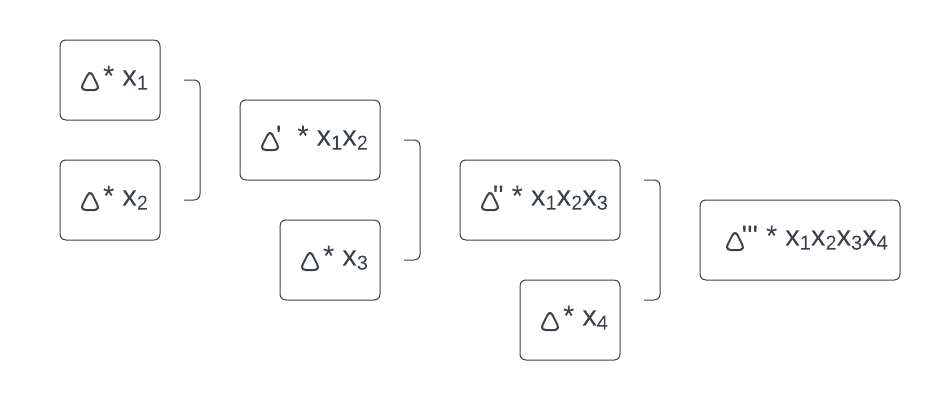
\includegraphics[scale = 0.75]{Blank diagram (2).png}
\end{center}

\subsection{Leveled HE}

% Homomorphic Operations of Ciphertexts at Different Levels. When given encryptions c, c′ of m, m′ belong to the different levels l and l′ < l, we should bring a ciphertext c at a larger level l to the smaller level l′ before homomorphic operation. There are two candidates: simple modular reduction and the RS procedure. It should be chosen very carefully
% by considering the scale of messages because the simple modular reduction c 7→ c (mod ql′ ) preserves the plaintext while RS procedure changes the plaintext from m to ql′ m as in Fig.3. ql Throughout this paper, we perform simple modulus reduction to the smaller modulus before computation on ciphertexts at different levels unless stated otherwise.

\noindent Ciphertexts might be at different levels while doing Homomorphic Operations. Before performing homomorphic operation, we should reduce a ciphertext's level from a bigger level $l$ to a smaller level $l'$ when the encryptions $c, c'$ of given messages $m, m'$ belong to distinct levels $l$ and $l'$. There are two contenders: the ReScaling technique and simple modular reduction. Since the ReScaling procedure changes $m$ to $\frac{q_{l'}}{q_l} m$, while the modular reduction $c \mapsto c$ (mod$ q_{l'}$) preserves the plaintext, it should be chosen very carefully. Unless otherwise mentioned, we compute on ciphertexts at various levels using simple modulus reduction to the smaller modulus throughout this study.
\\

\noindent Instead of doing linear multiplication of encrypted data we should perform the multiplication in a tree based structure. In linear multiplication we will need to perform $(n - 1)$ rescaling operations for $n$ multiplications on encrypted data. Instead we can perforn same number of multiplications in (log$n$ + 1) rescaling operations using tree based structure.

\begin{center}
    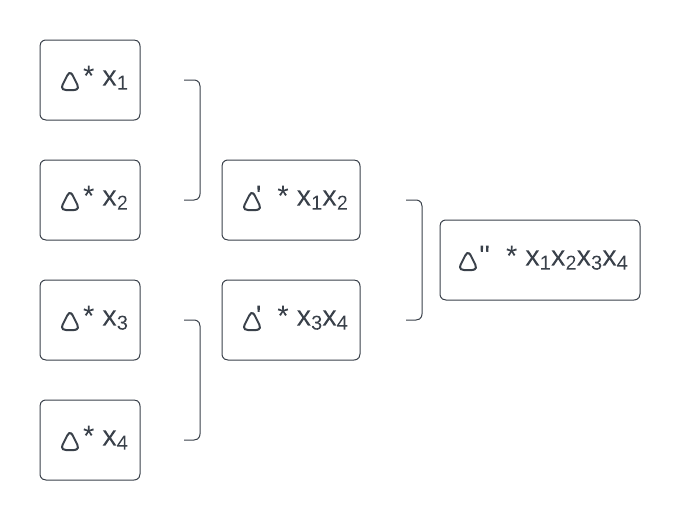
\includegraphics[width = 3 in]{Blank diagram (1).png}
\end{center}

\section{Credit Card Fraud Detection using HE}

\subsection{About Dataset}

In our credit card dataset, we have total 284808 rows and 31 columns from which, only transaction and amount columns are original, due of privacy concerns, all additional columns are scaled. The transactions aren't very big, really. The average of all the mounts produced is about 88. There are only 492 instances of Fraud transactions that is 0.17\%, all other transactions are Non-Fraud transactions that is 99.83\%. That also means that dataset is heavily imbalanced. Scaling has done by using PCA transformation(Dimensionality Reduciton Technique).

\begin{figure}[!h]
\centering
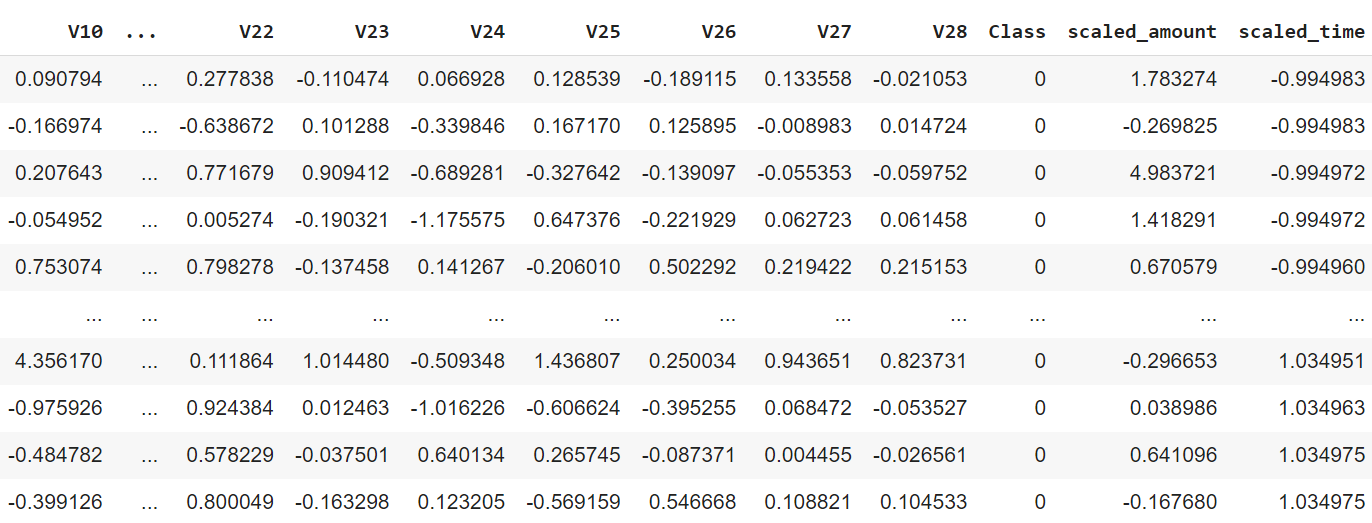
\includegraphics[width = 4 in]{img1.png}~
\end{figure}

\subsection{Preprocessing}

Since our dataset is very imbalanced, if we use this dataset for model training, it will not give very accurate results and can get many errors. Since most of them are non-fraud, Our model will operate on the presumption that the majority of transactions are non-fraud, thus it won't be able to spot the patterns that indicate a transaction is fraudulent.

\subsubsection{Scaling:}
We'll start by scaling the time and money column, which needs to be scaled similarly to the other columns. Because these values have a large range of values due to which the prediction will not be accurate so we need to scailing them in small range. Below is the code for scailing.\\

\noindent\textbf{CODE:}
\begin{figure}[!h]
\centering
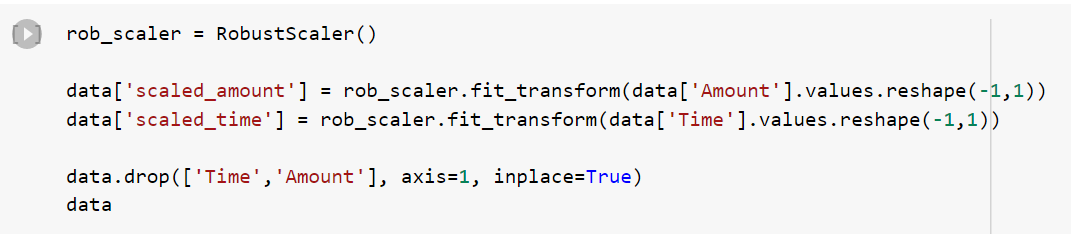
\includegraphics[width = 4.5 in]{img14.png}~
\end{figure}


% scailing code

\subsubsection{Distributing:}
We will create a sub-sample on which we can do model training to avoid overfitting, wrong correlations and imbalance. For that we will take 5:5 ratio of (Same amount) both class).\\

\noindent\textbf{CODE:}
\begin{figure}[!h]
\centering
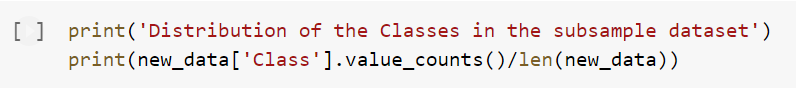
\includegraphics[width = 4.5 in]{img15.png}~
\end{figure}

% distributed code

\subsubsection{Random Under Sampling:}
To create a sub sample data frame, we will use random under sampling, in which we will choose the class which have less instances and will take the same amount of instances of other class.\\
So we will create a new sub-sample by concat 500 cases of 1st class and 500 transaction of 2nd class and then will shuffle the data. \textbf{Risk: Information Loss.}

% random sampling code
\noindent\textbf{CODE:}
\begin{figure}[!h]
\centering
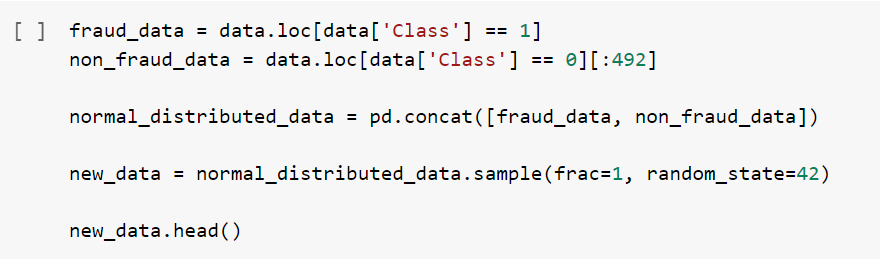
\includegraphics[width = 3.5 in]{img16.png}~
\end{figure}


\subsection{Analysis ( After Preprocessing) }

After preprocessing, we will observe the correlation between features and will also see the boxplots of theirs.

\subsubsection{Correlation Matrices:}
By using correlation matrices, we can observe that which features are heavily related with transaction being fraud. So we will use this matrix in sub-sample data frame and will see which features are positively correlated with fraud transactions and which are negatively correlated with fraud transactions.\\
We have observed that features V14 and V12's correlation is negative with fraud transactions so as the value of these features will be lower, the higher chance that transaction will be fraud.\\
We have also observed that V4 and V11's correlation is positive with fraud transactions so as the value of these features will be higher, the higher chance that transactions will be fraud.

\begin{figure}[!h]
\centering
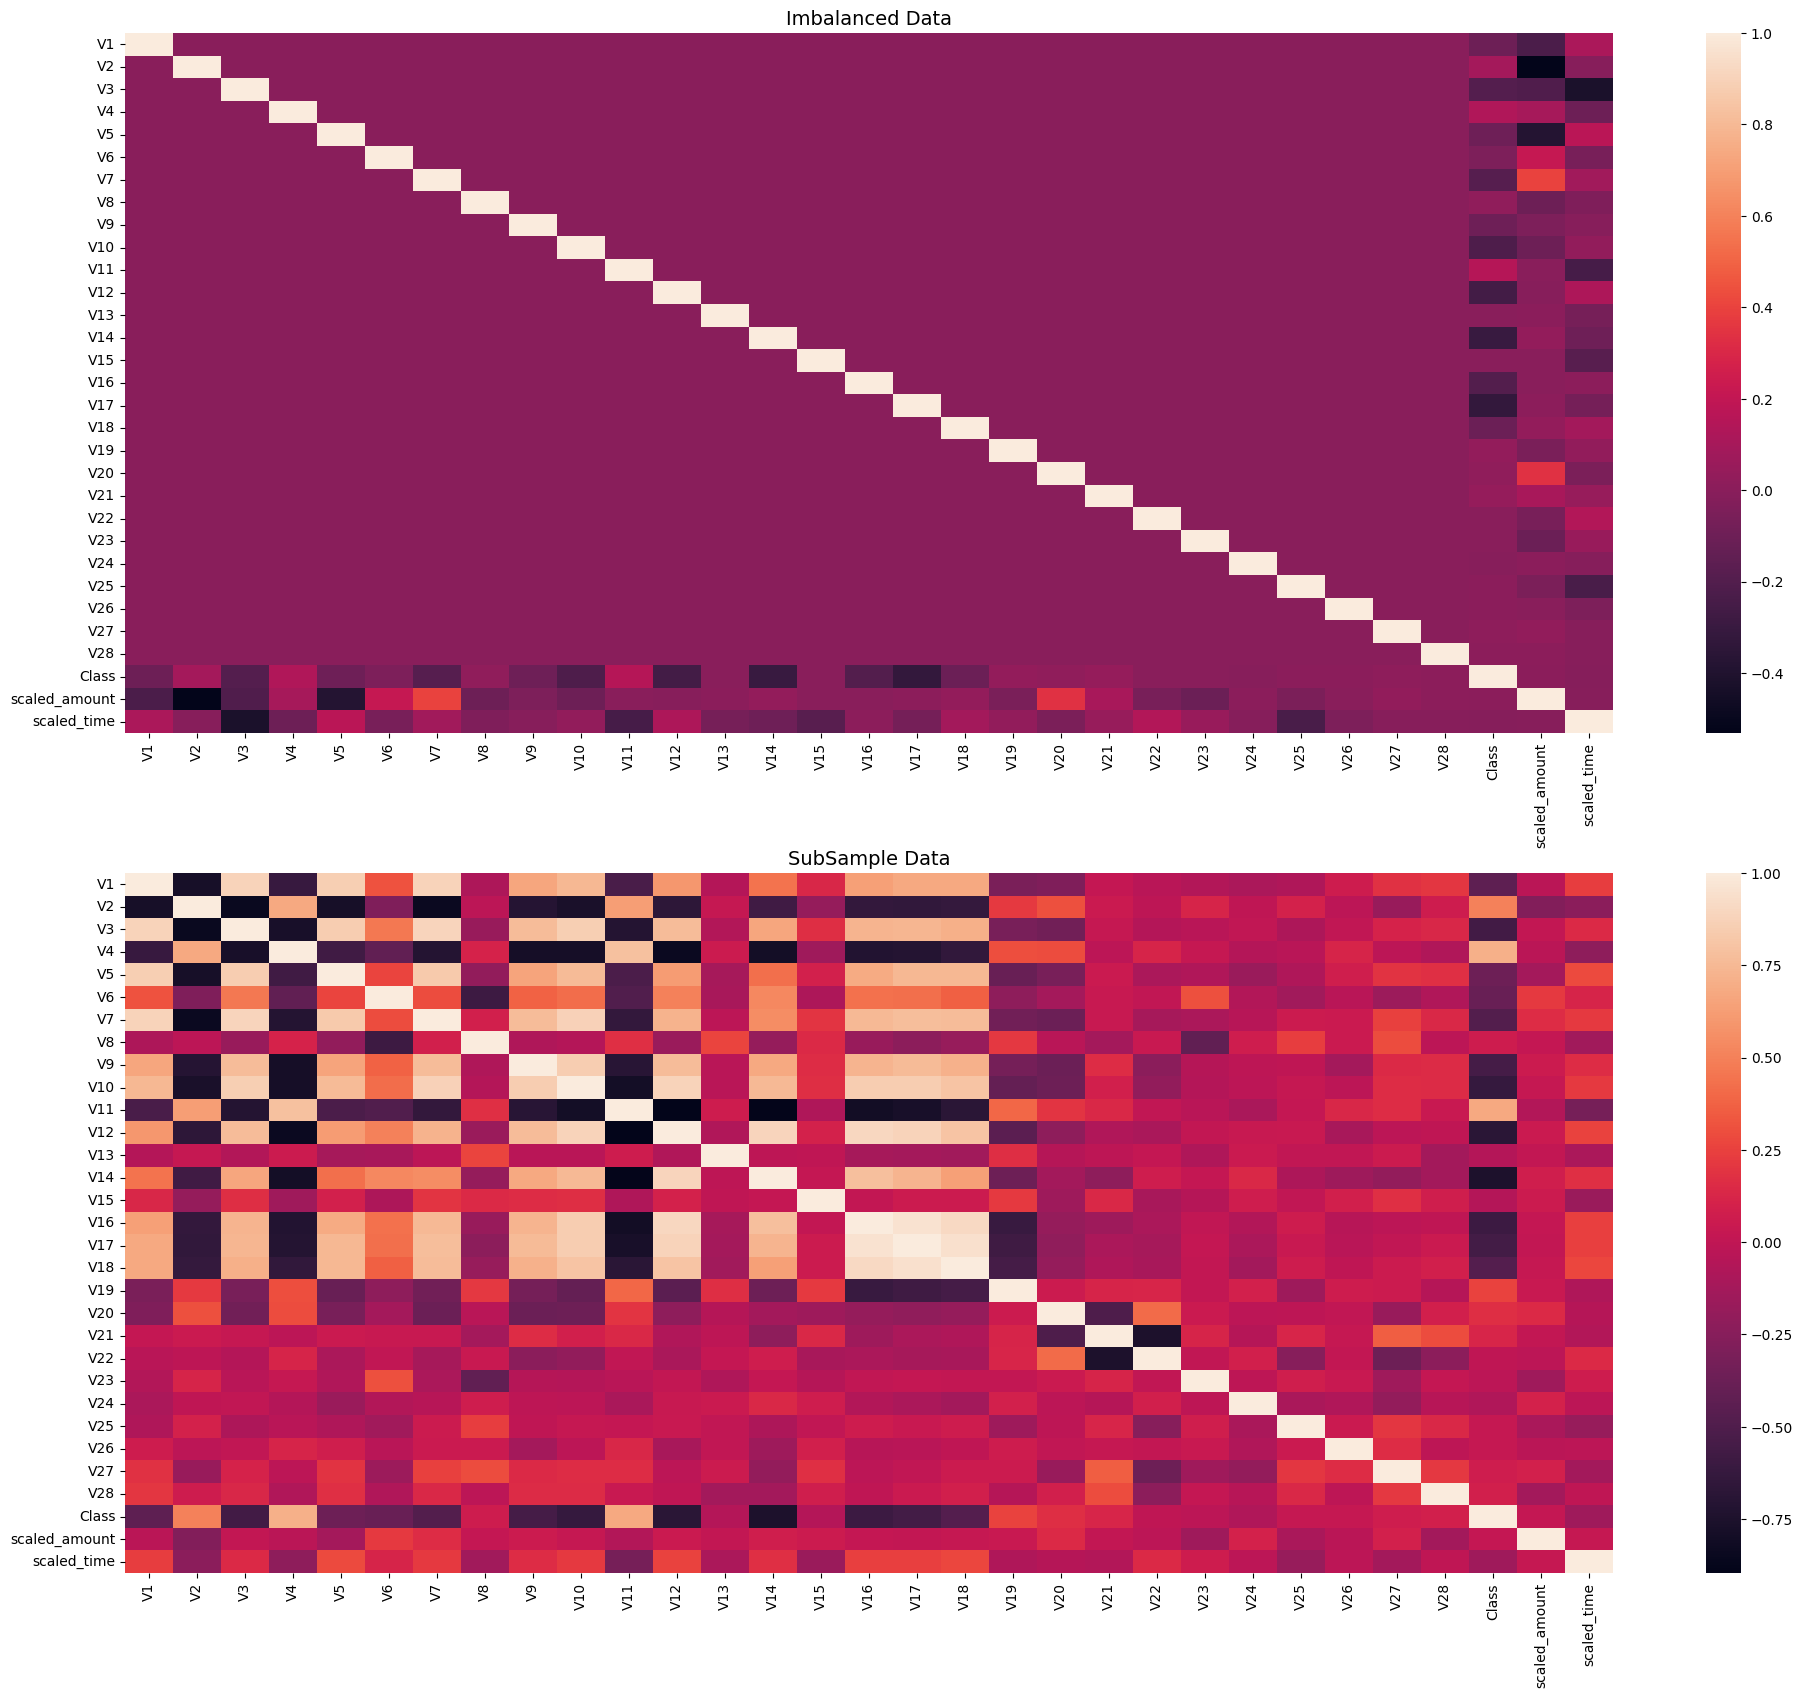
\includegraphics[width = 4 in]{img2.png}~
\end{figure}

\subsubsection{Box Plots:}
Box plots help us comprehend the features and how they are distributed in both fraudulent and legitimate transactions.\\
Here are some of the box plots of some features with class negative and class positive correlation.

\begin{figure}[!h]
\centering
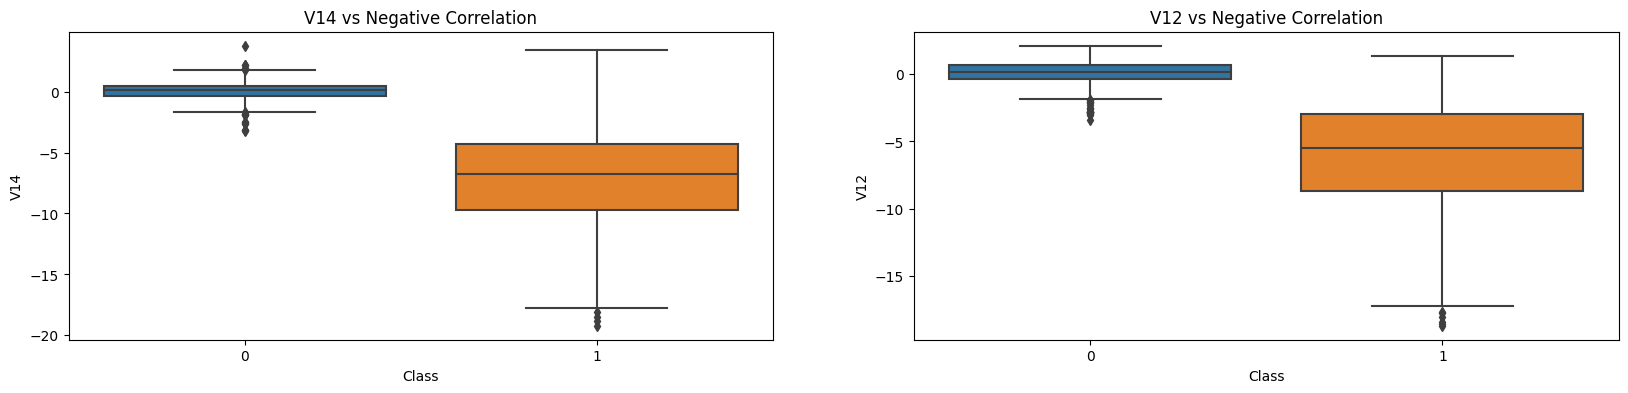
\includegraphics[width = 4 in]{img3.png}~
\end{figure}

\begin{figure}[!h]
\centering
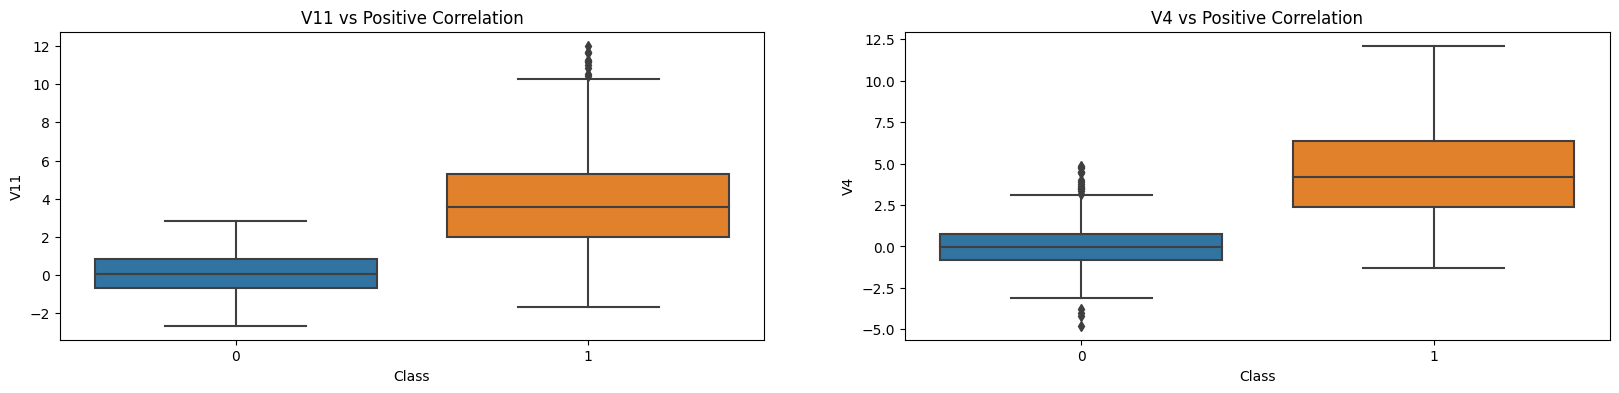
\includegraphics[width = 4 in]{img4.png}~
\end{figure}

\subsubsection{Outlier Removal:}
We need to remove the outliers from all the features which have very great amount of positive or negative correlation with fraud and non-fraud classes. By using this we can improve our accuracy of the model. For this we can use IQR to calculate the 25th and 75th percentile and can remove the transactions which are beyond the 25th and 75th percentile as an extreme outliers.\\

\begin{figure}[!h]
\centering
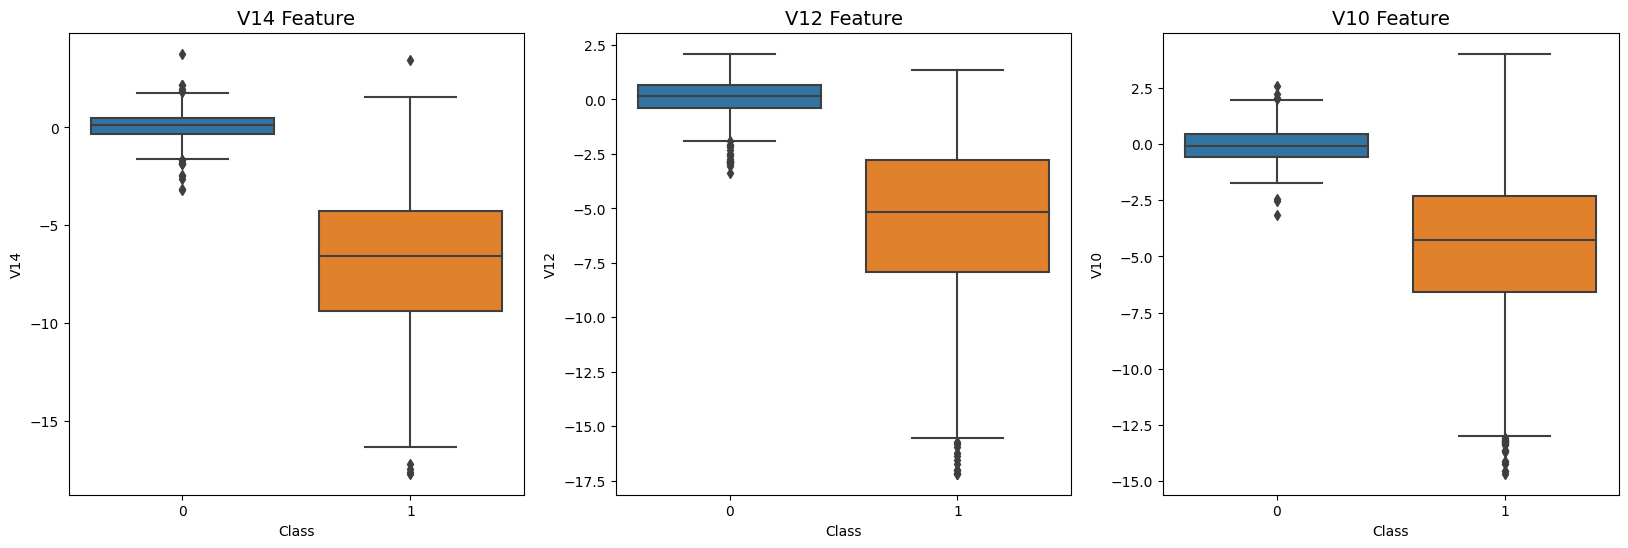
\includegraphics[width = 4 in]{img6.png}~
\end{figure}

\noindent\textbf{Tradeoff} is that We must be careful when deciding how far to raise the outlier removal threshold. The threshold is calculated by multiplying a value (for example, 3/2) by the inter-quartile range.On the other hand if multiplied by a larger value, such as three, it will discover fewer outliers; conversely, if this threshold is lower, it will detect more outliers and if it will detect more outliers, it might be risky because by doing that we can also lose some important pieces of information and by doing that we will have lower accuracy.

\subsubsection{Distribution plot:}
The distribution of the characteristic we will use to weed out some of the outliers is first visualised. Only feature V14 shows a Gaussian distribution in comparison to features V12 and V10.

\begin{figure}[!h]
\centering
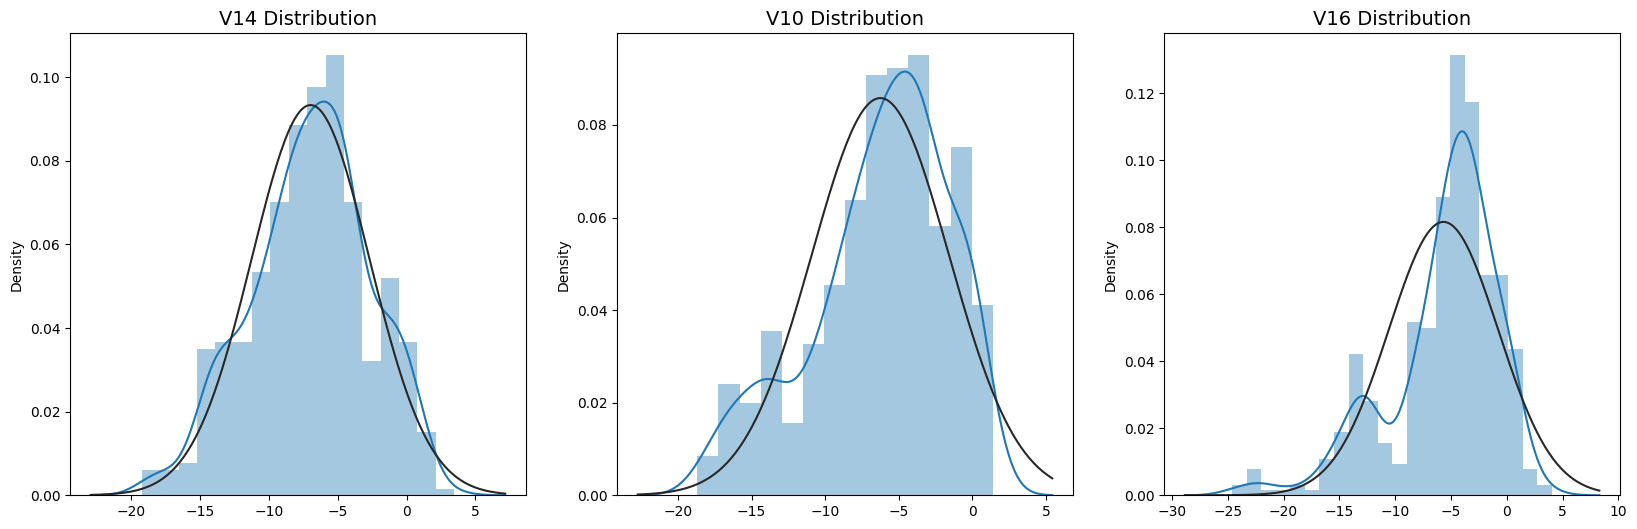
\includegraphics[width = 4 in]{img5.png}~
\end{figure}

\subsubsection{Threshold:}
The upper thresholds will be determined by adding the 75th quantile and the lower thresholds will be determined by subtracting 25th quantile after choosing the value that will be multiplied by the iqr.\\
We have also plot the graph that shows that after doing this, the number of outliers have decreased with considerable amount.\\
We have also observed that our accuracy has also i by 3\% though some outliers have distort the accuracy of out model.

\subsubsection{Clustering and PCA:}
We will use PCA (Dimensionality Reduction) to reduce the dimension of our data and then we will use clustering to see how well our model will separate two classes(fraud and non-fraud).\\
We have observed that PCA has done very good clustering of both classes in our dataset. Even though the sub-sample was pretty small. So we can also tell that further models that we will apply will also perform well.

\begin{figure}[!h]
\centering
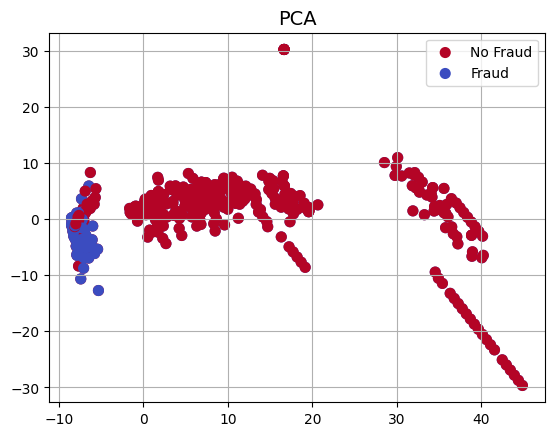
\includegraphics[width = 2.33 in]{img7.png}~
\end{figure}

\subsection{Model Training (Logistic Regression):}
For training out data set, we have used Logistic Regression model.Before that,Additionally, the dataset has been divided into training and testing sets. In order to anticipate it, we have additionally separated the labels from other features.

\subsubsection{Observation:}
We have observed that, our model is more likely to be overfitted (have a high variance) if the training score and the cross-validation score differ significantly.\\
Our model is underfitting (high bias) if the score is low in both the training and cross-validation sets.\\
The results of logistic regression are excellent in both the cross-validating as well as training sets.\\
Following is the plot of the \textbf{Learning curve of Logistic regression.}
\\\\

\begin{figure}[!h]
\centering
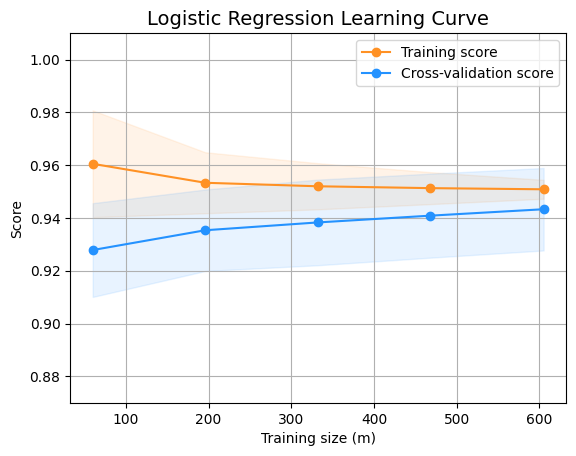
\includegraphics[width = 2.8 in]{img8.png}~
\end{figure}

\subsubsection{Confusion matrix:}
\textbf{True Positive(tp):} Transactions Classified As Fraud Correctly\\
\textbf{False Positive(fp):} Incorrectly Classified Fraud Transactions\\
\textbf{True Negative(tn):} Transactions Classified Non-Fraud Correctly\\
\textbf{False Negative(fn):} Incorrectly Classified Non-Fraud Transactions\\
\textbf{Precision:} tp / ( tp + fp )\\
\textbf{Recall:} tp / (tp + fn )\\

\noindent\textbf{Precision and Recall Tradeoff:} Our model will find fewer examples as it becomes more Precise(selective). Example: Let's assume that the model has a 95\% accuracy rate, let's say that there are only 5 instances of fraud for which the model has an accuracy rate of 95\% or higher. If we lower the precision, our model will be able to discover more cases, such as the additional 5 cases that our model believes to be 90\% fraud cases.


\section{Encryption Process}

\subsection{Flowchart of model using plain data}

The below image shows the whole process of how and where the model is trained and where we are doing the encryption.

\begin{figure}[!h]
\centering
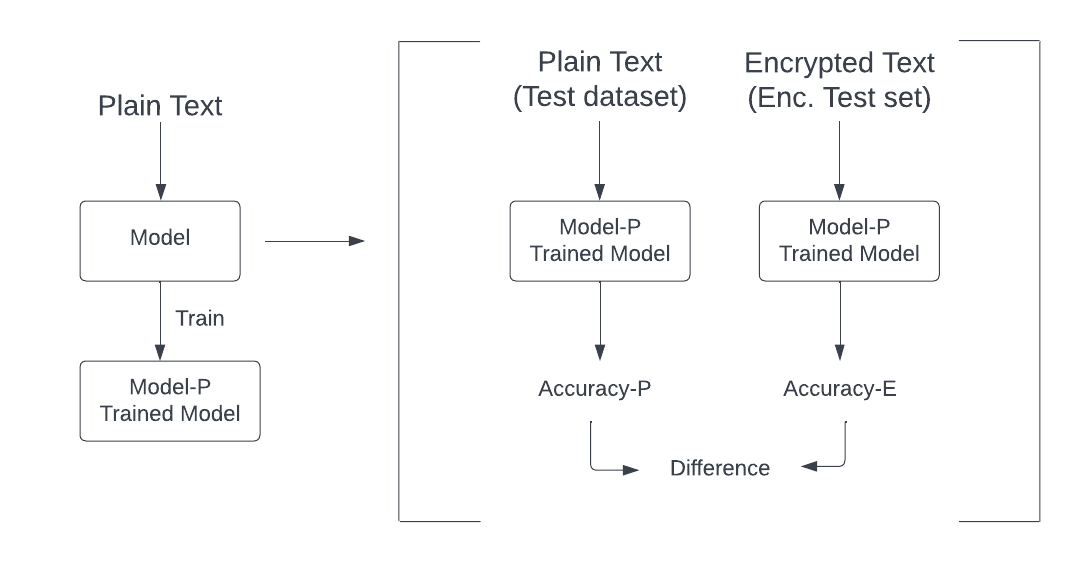
\includegraphics[width = 4 in]{img12.png}~
\end{figure}

\subsection{Logistic Model on Plain Train\_Set}

\begin{itemize}
\item First we have trained our model on plain text 5 times using Logistic Regression  Gradient Descent.

\item After that we have calculated the loss at each iteration and observed that after each iteration the loss was decreasing because each time when we were getting parameters, we were using it as initial value for next iteration.
 
\end{itemize}

% Loss at each iteration
\begin{figure}[!h]
\centering
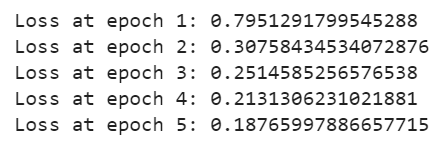
\includegraphics[width = 2.8 in]{img13.png}~
\end{figure}

% slide 37
\begin{itemize}
\item Then after training the model we have calculated the accuracy on plain test set.

\begin{figure}[!h]
\centering
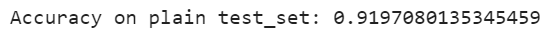
\includegraphics[width = 3 in]{img17.png}~
\end{figure}

\item Now we have encrypted the test data and calculated the accuracy on cipher test set

\begin{figure}[!h]
\centering
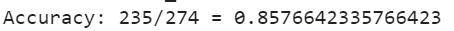
\includegraphics[width = 3 in]{img17a.png}~
\end{figure}

\item Difference between the accuracy of plain and cipher test set

\begin{figure}[!h]
\centering
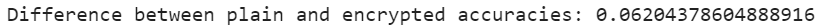
\includegraphics[width = 4 in]{img17b.png}~
\end{figure}
 
\end{itemize}


\subsection{Flowchart of Model using Encrypted Data}
\begin{figure}
\centering
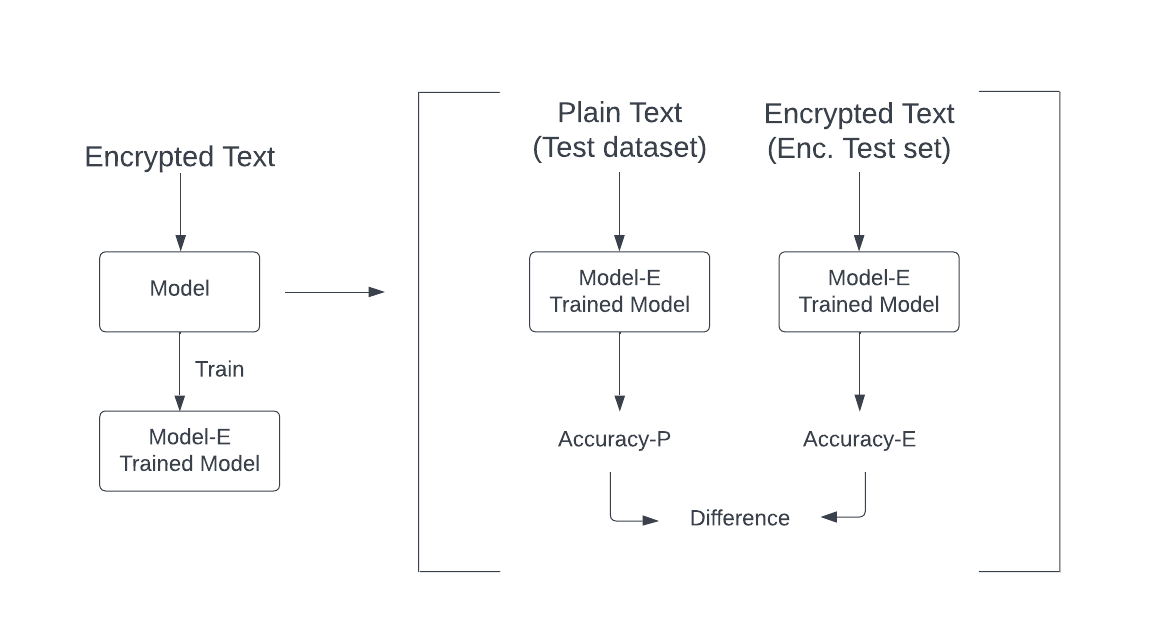
\includegraphics[width = 4 in]{img11.png}~
\end{figure}

\subsection{Two types of process happening in Model}

% slide 39
\begin{figure}[!h]
\centering
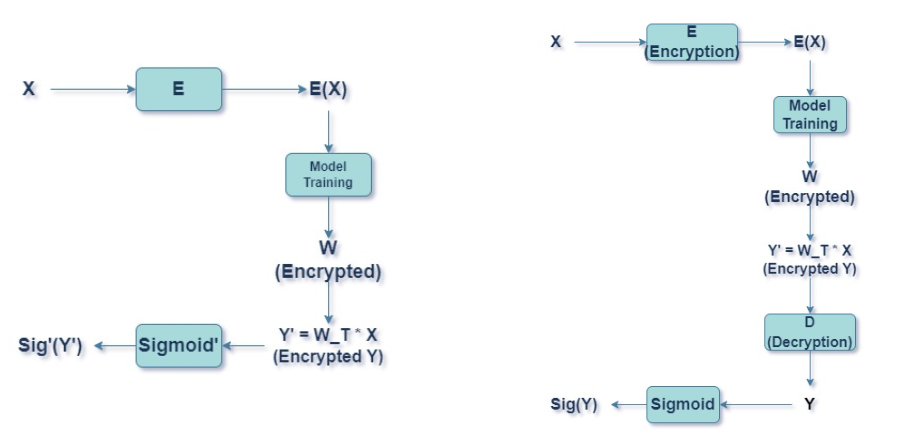
\includegraphics[width = 4 in]{img18.png}~
\end{figure}

\begin{itemize}
\item Here first of all we have encrypted our train set.

\item Then we have trained our model on cipher train set 5 times using Logistic Regression \& Gradient Descent.

\item After getting the optimal parameter values we have calculated the accuracy of cipher test set using different sigmoid function and then using the parameters we have predicted the class on plain test set and decrypted the result because those are encrypted results
    
\item And after decrypting the result we have calculated the accuracy and found the difference between the accuracies

\end{itemize}

\begin{figure}[!h]
\centering
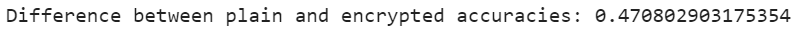
\includegraphics[width = 4.3in]{img19.png}~
\end{figure}
\newpage

Here are the references \cite{nugent2022privacy} , \cite{cheon2017homomorphic}

\bibliographystyle{alpha}
\bibliography{references}

\end{document}
